\chapter{Analiza ruchu robota}
Najczęściej spotykanym modelem odwróconego wahadła jest wahadło umieszczone na poruszającym się w jednej osi wózku, a rolę sterowania odgrywa siła przyłożona do wózka równolegle do kierunku ruchu. W omawianym w tym rozdziale przypadku rolę wózka odgrywa podwozie wyposażone w koła, a siłą sterującą jest moment obrotowy oddziałujący na wahadło. Różnice pomiędzy tymi modelami, przedstawione są na schemacie \ref{Modele odwroconego wahadla}

    \begin{figure}[h!]
	    \centering
	    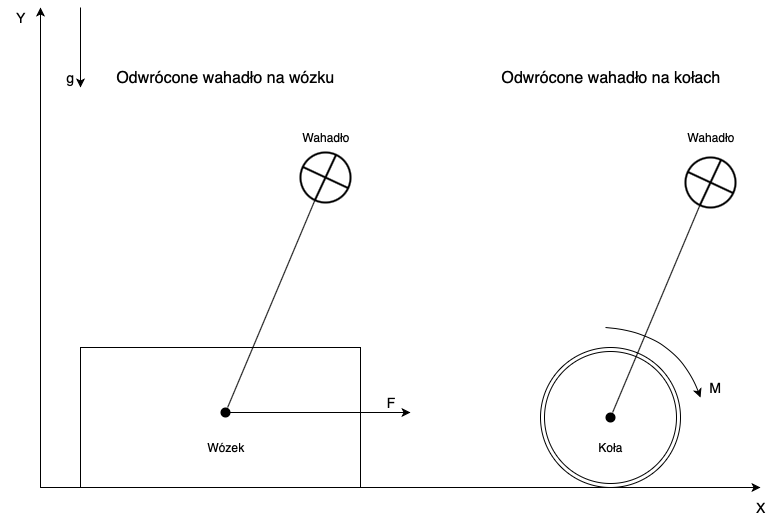
\includegraphics[width=0.75\textwidth]{Rysunki/Rozdzial02/Schemat_wozek_kola.png}
	    \caption{Modele odwróconego wahadła}
	    \label{Modele odwroconego wahadla}
	\end{figure}

\section{Model dynamiki robota balansującego}

W celu ułatwienia implementacji algorytmu sterującego na rzeczywistym robocie, wyprowadzone zostały jego równania dynamiki oraz równania stanu pozwalające na przetestowanie układu sterowania w środowisku \texttt{Matlab Simulink}. W modelu pominięto opory powietrza oraz tarcie pomiędzy wahadłem a kołami oraz kołami a podłożem. Prędkości oraz siły w układzie zostały przedstawione na schemacie \ref{Schemat modelu}

    \begin{figure}[h!]
	    \centering
	    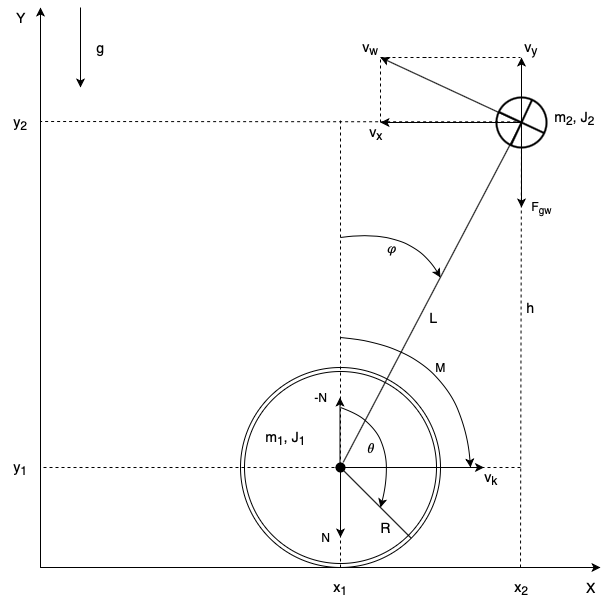
\includegraphics[width=0.75\textwidth]{Rysunki/Rozdzial02/Schemat_modelu_dynamiki.png}
	    \caption{Schemat modelu}
	    \label{Schemat modelu}
	\end{figure}
	
	\newpage
	
Oznaczenia występujące na schemacie modelu dynamiki, przedstawione są w tabeli:
    \begin{table}[h!]
        \centering
        \caption{Oznaczenia wykorzystywane w modelu}
        \label{Oznaczenia}
        \begin{tabular}{|c|l|}
              \hline
              Symbol & Opis\\
              \hline
              $\varphi$ & Kąt wychylenia wahadła od pionu \\
              \hline
              $\theta$ & Kąt obrotu koła względem pionu \\
              \hline
              $x_1, y_1$ & Współrzędne środka połączenia koła z wahadłem \\
              \hline
              $x_2, y_2$ & Współrzędne środka masy wahadła \\
              \hline
              $m_1$ & Masa koła \\
              \hline
              $m_2$ & Masa wahadła \\
              \hline
              $J_1$ & Moment bezwładności koła \\
              \hline
              $J_2$ & Moment bezwładności wahadła \\
              \hline
              $R$ & Promień koła \\
              \hline
              $M$ & Moment siły generowany przez napęd\\
              \hline
              $L$ & Odległość środka masy wahadła od osi obrotu \\
              \hline
              $h$ & Wysokość na jakiej znajduje się środek masy wahadła \\
              \hline
              $g$ & Wektor siły grawitacji \\
              \hline
              $F_{gw}$ & Wektor siły ciężkości oddziałującej na środek masy wahadła \\
              \hline
              $N$ & Wektor siły nacisku koła na podłoże \\
              \hline
              $v_w, v_x, v_x $ & Wektory prędkości środka masy wahadła \\
              \hline
              $v_k$ & Wektor prędkości koła \\
              \hline
        \end{tabular}
    \end{table}
    	
Parametry obiektu eksperymentalnego wykorzystane podczas symulacji i obliczeń:
    \begin{table}[h!]
        \centering
        \caption{Parametry modelu}
        \label{Parametry}
        \begin{tabular}{|c|c|c|}
              \hline
              Symbol & Wartość & Jednostka\\
              \hline
              $m_1$ & $0,02$ & $kg$\\
              \hline
              $m_2$ & $1,2$ & $kg$\\
              \hline
              $R$ & $0,04$ & $m$\\
              \hline
              $L$ & $0,05$ & $m$\\
              \hline
              $J_1$ & $\frac{1}{2}\cdot m_1 \cdot R^2 = 0,000026$ & $kg \cdot m^2$\\
              \hline
              $J_2$ & $\frac{1}{3}\cdot m_2 \cdot L^2 = 0,002$ & $kg \cdot m^2$\\
              \hline
              $g$ & $9,806$ & $\frac{m}{s^2}$\\
              \hline
        \end{tabular}
    \end{table}

Korzystając z funkcji trygonometrycznych i zależności pomiędzy odległością środka masy wahadła od jego początku oraz kątem zakreślonym przez wahadło, można wyznaczyć położenie środka masy wahadła w zależności od położenia środka koła. Dodatkowo wysokość na jakiej znajduje się środek koła, jest jednocześnie jego promieniem $y_2 = R$. Współrzędne środka masy wahadła:
$$
    \left\{
    \begin{array}{lr}
    \frac{x_2-x_1}{L} = sin\varphi \\
    \frac{y_2-y_1}{L} = cos\varphi
    \end{array}
    \right.
    \Rightarrow
    \left\{
    \begin{array}{lr}
    x_2 = x_1 + Lsin\varphi \\
    y_2 = y_1 + Lcos\varphi
    \end{array}
    \right.
    \Rightarrow
    \left\{
    \begin{array}{lr}
    x_2 = x_1 + Lsin\varphi \\
    y_2 = R + Lcos\varphi
    \end{array}
    \right.
$$

Korzystając z twierdzenia odwrotnego do twierdznia Pitagorasa, oraz rachunku różniczkowego (prędkość jako pochodna po czasie z przebytej drogi) można wyznaczyć prędkość środka masy wahadła na podstawie jej składowych w osi x oraz y. Składowe prędkości jako pochodne z przemieszczenia w osi x oraz y
$$
    \left\{
    \begin{array}{c}
    \dot{x}_2 = \dot{x}_1 + Lcos\varphi\dot{\varphi} \\
    \dot{y}_2 = -Lsin\varphi\dot{\varphi}
    \end{array}
    \right.
$$
oraz prędkość wypadkowa wahadła obliczona przy wykorzystaniu twierdzenia odwrotnego do twierdzenia Pitagorasa:
\begin{equation}
    \begin{array}{ll}
    v_w^2 = v_x^2 + v_y^2 \Rightarrow v_w = \sqrt{\dot{x}_2^2 + \dot{y}_2^2} \\ \\
    v_w = \sqrt{\dot{x}_1^2 + 2\dot{x}_1Lcos\varphi\dot{\varphi} + L^2cos^2\varphi\dot{\varphi}^2 + L^2sin^2\varphi\dot{\varphi}^2} = \sqrt{\dot{x}_1^2 + 2\dot{x}_1Lcos\varphi\dot{\varphi} + L^2\dot{\varphi}^2}
    \end{array}
\end{equation}

%---------------------------------------------------------------------------------------------
\subsection{Energia kinetyczna}
Znając prędkość wypadkową wahadła, wyznacza się jego energię kinetyczną, która jest sumą energii kinetycznej ruchu postępowego i energii kinetycznej ruchu obrotowego
$$
    \begin{array}{ll}
    K_w = \frac{1}{2}m_2v_w^2 + \frac{1}{2}J_2\dot{\varphi}^2 = \frac{1}{2}m_2(\dot{x}_1^2 + 2\dot{x}_1Lcos\varphi\dot{\varphi} + L^2\dot{\varphi}^2) + \frac{1}{2}J_2\dot{\varphi}^2
    \end{array}
$$
oraz w analogiczny sposób wyznacza się energię kinetyczną koła
$$
    \begin{array}{ll}
    K_k = \frac{1}{2}m_1\dot{x}_1^2 + \frac{1}{2}J_1\dot{\theta}^2
    \end{array}
$$

Energia kinetyczna układu jest sumą energii kinetycznej wahadła oraz dwóch kół:
\begin{equation}
    \begin{array}{ll}
    K = K_w + 2K_k = \frac{1}{2}m_2(\dot{x}_1^2 + 2\dot{x}_1Lcos\varphi\dot{\varphi} + L^2\dot{\varphi}^2) + \frac{1}{2}J_2\dot{\varphi}^2 + m_1\dot{x}_1^2 + J_1\dot{\theta}^2
    \end{array}
\end{equation}

%---------------------------------------------------------------------------------------------
\subsection{Energia potencjalna}

Środek masy wahadła znajduje się na wysokości $y_2 = m_2g(R + Lcos\varphi)$, a po wstawieniu jej do wzoru na energię potencjalną ciała o masie $m$ znajdującego się na wysokości $h$, otrzymujemy energię potencjalną środka masy wahadła:
$$
    \begin{array}{ll}
    V_w = mgh = m_2gy_2 = m_2g(R + Lcos\varphi)
    \end{array}
$$

Energia potencjalna koła:
$$
    \begin{array}{ll}
    V_k = m_1gR
    \end{array}
$$

Gdyby przyjęto układ współrzędnych, w którym środek koła znajdowałby się na wysokości $y_2 = 0$, to energia potencjalna koła wynosiłaby 0. \\

Energia potencjalna układu jest sumą energii potencjalnej w środku masy wahadła, oraz energii potencjalnej dwóch kół:
\begin{equation}
    \begin{array}{ll}
    V = V_w + 2V_k = m_2g(R + Lcos\varphi) + 2m_1gR
    \end{array}
\end{equation}

%---------------------------------------------------------------------------------------------
\subsection{Równania Eulera--Lagrange'a}

Znając energię kinetyczną oraz potencjalną układu przystąpić można do obliczenia Lagranżjanu \cite{ManipulatoryiRoboty}, który jest różnicą energii kinetycznej oraz potencjalnej układu
\begin{equation}
    \begin{array}{cl}
    \mathcal{L} = K - V \\ \\ 
    \mathcal{L} = \frac{1}{2}m_2(\dot{x}_1^2 + 2\dot{x}_1Lcos\varphi\dot{\varphi} + L^2\dot{\varphi}^2) + m_1\dot{x}_1^2 + J_1\dot{\theta}^2 - m_2g(R + Lcos\varphi) - 2m_1gR
    \label{Lagranżjan}
    \end{array}
\end{equation}
gdzie droga przebyta przez toczące się koło oraz prędkość ruchu postępowego wynosi $x_1 = R\theta$, a co za tym idzie prędkość koła w osi x to $\dot{x}_1 = R\dot{\theta}$, co po wstawieniu do wzoru (\ref{Lagranżjan}) daje ostateczną postać Lagrangianu:
\begin{equation}
    \begin{array}{ll}
    \mathcal{L} = \frac{1}{2}m_2(R^2\dot{\theta}^2 + 2R\dot{\theta}Lcos\varphi\dot{\varphi} + L^2\dot{\varphi}^2) + m_1R^2\dot{\theta}^2 + \\ \\
    + J_1\dot{\theta}^2 - m_2g(R + Lcos\varphi) - 2m_1gR
    \end{array}
\end{equation}

Mając dany Lagranżjan, przystępujemy do wyznaczenie równań Eulera-Lagrange'a drugiego rodzaju, których ogólna postać wygląda następująco
$$
    \begin{array}{ll}
    \frac{d}{dt}\frac{\delta\mathcal{L}}{\delta\dot{q_i}} - \frac{\delta\mathcal{L}}{\delta q_i} = F_i
    \end{array}
$$
gdzie
\begin{itemize}
    \item $\frac{\delta\mathcal{L}}{\delta q_i}$ -- i-ta składowa siły uogólnionej
    \item $\frac{\delta\mathcal{L}}{\delta\dot{q_i}}$ -- i-ta składowa pędu uogólnionego
    \item $F_i$ -- i-ta składowa sił niepotencjalnych
\end{itemize}

W tym przypadku składowe dla zmiennych $\varphi$ oraz $\theta$ wynoszą odpowiednio
$$
    \varphi:
    \left\{
    \begin{array}{ll}
    \frac{\delta\mathcal{L}}{\delta\varphi} = -m_2R\dot{\theta}Lsin\varphi\dot{\varphi}
    \frac{\delta\mathcal{L}}{\delta\dot{\varphi}} = m_2R\dot{\theta}Lcos\varphi + m_2L^2\dot{\varphi} + J_2\dot{\varphi}
    \end{array}
    \right.
$$

$$
    \theta:
    \left\{
    \begin{array}{ll}
    \frac{\delta\mathcal{L}}{\delta\theta} = 0 \\ \\
    \frac{\delta\mathcal{L}}{\delta\dot{\theta}} = m_2R^2\dot{\theta} + m_2RLcos\varphi\dot{\varphi} + 2m_1R^2\dot{\theta} + 2J_1\dot{\theta} 
    \end{array}
    \right.
$$

Mając wszystkie składowe oblicza się jeszcze pochodne po czasie składowych sił uogólnionych i otrzymujemy ostatecznie równania Eulera-Lagrange'a:
\begin{equation}
    \begin{array}{ll}
    \frac{d}{dt}\frac{\delta\mathcal{L}}{\delta\dot{\varphi}} - \frac{\delta\mathcal{L}}{\delta\varphi} = m_2R\Ddot{\theta}Lcos\varphi - m_2R\dot{\theta}sin\varphi\dot{\varphi} + m_2L^2\Ddot{\varphi} + J_2\Ddot{\varphi} + m_2R\dot{\theta}Lsin\varphi\dot{\varphi} + \\ \\
    - m_2gLsin\varphi = m_2R\Ddot{\theta}Lcos\varphi + m_2L^2\Ddot{\varphi} + J_2\Ddot{\varphi} - m_2gLsin\varphi = -M
    \\ \\
    \frac{d}{dt}\frac{\delta\mathcal{L}}{\delta\dot{\theta}} - \frac{\delta\mathcal{L}}{\delta\theta} = m_2R^2\Ddot{\theta} - m_2RLsin\varphi\dot{\varphi}^2 + m_2RLcos\varphi\Ddot{\varphi} + 2m_1R^2\Ddot{\theta} + 2J_1\Ddot{\theta} = M
    \end{array}
\end{equation}
%
gdzie $M$ to moment siły generowany przez napęd. Dla zmiennej $\theta$ ze znakiem dodatnim, ponieważ kierunek obrotu kół jest zgodny z kierunkiem generowanego momentu. Dla zmiennej $\varphi$ z ujemnym znakiem, ponieważ kierunek obrotu wahadła jest przeciwny do działającego momentu siły. 

Równania dynamiki można przedstawić w postaci macierzowej, która jest bardziej czytelna
$$
    \begin{array}{cc}
        \left[ \begin{array}{cc}
        m_2L^2 + J_2 & m_2RLcos\varphi \\
        m_2RLcos\varphi & m_2R^2 + 2m_1R^2 + 2J_1
        \end{array} \right]
        \left[ \begin{array}{c}
        \Ddot{\varphi} \\
        \Ddot{\theta}
        \end{array} \right]
        +
        \left[ \begin{array}{cc}
        0 & 0 \\
        -m_2RLsin\varphi\dot{\varphi} & 0
        \end{array} \right]
        \left[ \begin{array}{c}
        \dot{\varphi} \\
        \dot{\theta}
        \end{array} \right]
        + \\ \\ +
        \left[ \begin{array}{c}
        -m_2gLsin\varphi \\
        0
        \end{array} \right]
        = 
        \left[ \begin{array}{c}
        -M \\
        M
        \end{array} \right]
    \end{array}
$$

Taki model jest jednak nieliniowy i liniowy algorytm sterowania nie zadziałałby dla niego poprawnie, dlatego dokonuje się częściowej linearyzacji modelu w okolicach punktu równowagi, w przypadku w którym chcemy wykorzystać liniowy sterownik. Jednym z punktów równowagi odwróconego wahadła jest jego pionowa pozycja, punkt niestabilny. Drugi punkt równowagi to swobodne zwisanie wahadła, który jest stabilnym punktem równowagi, jednak zostaje on pominięty ze względu na jego brak w rozważanym modelu. Dla punktu równowagi $\varphi \approx 0$ możemy dokonać linearyzacji modelu dla którego
$$
    \left\{
    \begin{array}{c}
    sin\varphi \approx \varphi, \\
    cos\varphi \approx 1, \\
    \dot{\varphi}^2 \approx 0
    \end{array}
    \right.
$$

i zapisać w postaci 
$$
M(q)\Ddot{q} + C(q,\dot{q})\dot{q} + D(q) = u 
$$

gdzie:
\begin{itemize}
    \item $q$ -- wektor uogólnionych współrzędnych,
    \item $\dot{q}$ -- wektor uogólnionych prędkości,
    \item $M(q)$ -- symetryczna, dodatnio określona macierz inercji,
    \item $C(q,\dot{q})$ -- macierz sił Coriolisa i sił dośrodkowych,
    \item $D(q)$ -- wektor oddziaływań potencjalnych,
    \item $u$ -- wektor sterowań.
\end{itemize}

$$
\mathbf{M(q)} =
\left[ \begin{array}{cc}
m_2L^2 + J_2 & m_2RL \\
m_2RL & m_2R^2 + 2m_1R^2 + J_1
\end{array} \right]
$$
\\
$$
\mathbf{C(q,\dot{q})} = \emptyset
$$
\\
$$
\mathbf{D(q)} =
\left[ \begin{array}{c}
-m_2gL \\
0
\end{array} \right]
$$
\\
$$
\mathbf{q} =
\left[ \begin{array}{c}
\varphi \\
\theta \\
\end{array} \right]
,
\mathbf{u} =
\left[ \begin{array}{c}
-M \\
M \\
\end{array} \right]
$$

%---------------------------------------------------------------------------------------------
\subsection{Równania stanu}

W celu łatwiejszego wyznaczenia równań stanu zapisujemy równania dynamiki w następującej formie macierzowej  
$$
E\Ddot{q} + F\dot{q} + Gq = Hu 
$$
w której poszczególne elementy są równe
$$
\mathbf{E} = 
\left[ \begin{array}{cc}
m_2L^2 + J_2 & m_2RL \\
m_2RL & m_2R^2 + 2m_1R^2 + J_1
\end{array} \right]
$$
\\
$$
\mathbf{F} = \emptyset
$$
\\
$$
\mathbf{G} = 
\left[ \begin{array}{cc}
-m_2gL & 0 \\
0 & 0
\end{array} \right]
$$
\\
$$
\mathbf{H} = 
\left[ \begin{array}{c}
-1 \\
1
\end{array} \right]
$$

Mnożąc lewostronnie powyższe równanie przez macierz $\mathbf{E^{-1}}$ i wyznaczając pochodne pierwszego i drugiego rzędu, można przystąpić do sformułowania równań stanu. Przyjmują one postać dwóch równań
\begin{equation}
    \left\{
    \begin{array}{ll}
    \dot{x} = Ax + Bu \\
    y = Cx + Du
    \end{array}
    \right.
\end{equation}
w których:
\begin{itemize}
    \item x -- wektor stanu
    \item y -- wektor wyjścia
    \item u -- wymuszenie
\end{itemize}

$$
\mathbf{x} =
\left[ \begin{array}{c}
\varphi \\
\theta \\
\dot{\varphi} \\
\dot{\theta}
\end{array} \right]
\Rightarrow
\mathbf{\dot{x}} =
\left[ \begin{array}{c}
\dot{\varphi} \\
\dot{\theta} \\
\Ddot{\varphi} \\
\Ddot{\theta}
\end{array} \right]
$$
\\ \\
$$
\mathbf{A} =
\left[ \begin{array}{c|ccc}
\begin{array}{cc}
0 & 0 \\
0 & 0
\end{array}
& 
\begin{array}{cc}
1 & 0 \\
0 & 1
\end{array} \\
\hline
-E^{-1}G & -E^{-1}F
\end{array} \right] 
,
\mathbf{B} =
\left[ \begin{array}{c}
0 \\
0 \\
-E^{-1}H
\end{array} \right] 
$$
\\ \\
$$
\mathbf{C} =
\left[ \begin{array}{cccc}
1 & 0 & 0 & 0 \\
0 & 1 & 0 & 0 \\
0 & 0 & 1 & 0 \\
0 & 0 & 0 & 1 \\
\end{array} \right] 
,
\mathbf{D} = \emptyset
, 
\mathbf{u} = M
$$

\newpage

%---------------------------------------------------------------------------------------------
\section{Sterowanie}
Jednym z najprostszych i najpopularniejszych algorytmów sterowania odwróconym wahadłem, jest wykorzystanie układu regulacji ze sprzężeniem zwrotnym oraz regulatora PID. Algorytm zaimplementowano i przetestowano w środowisku \texttt{Matlab Simulink}.

%---------------------------------------------------------------------------------------------
\subsection{Pojedynczy regulator PID}
Zadaniem algorytmu jest utrzymanie wychylenia wahadła w okolicy punktu równowagi, dlatego w takim przypadku jest to układ dosterowany (jedna wielkość regulowana i jedno wymuszenie) i w zupełności wystarczy układ regulacji z pojedynczym regulatorem PID.
\begin{figure}[h!]
    \centering
	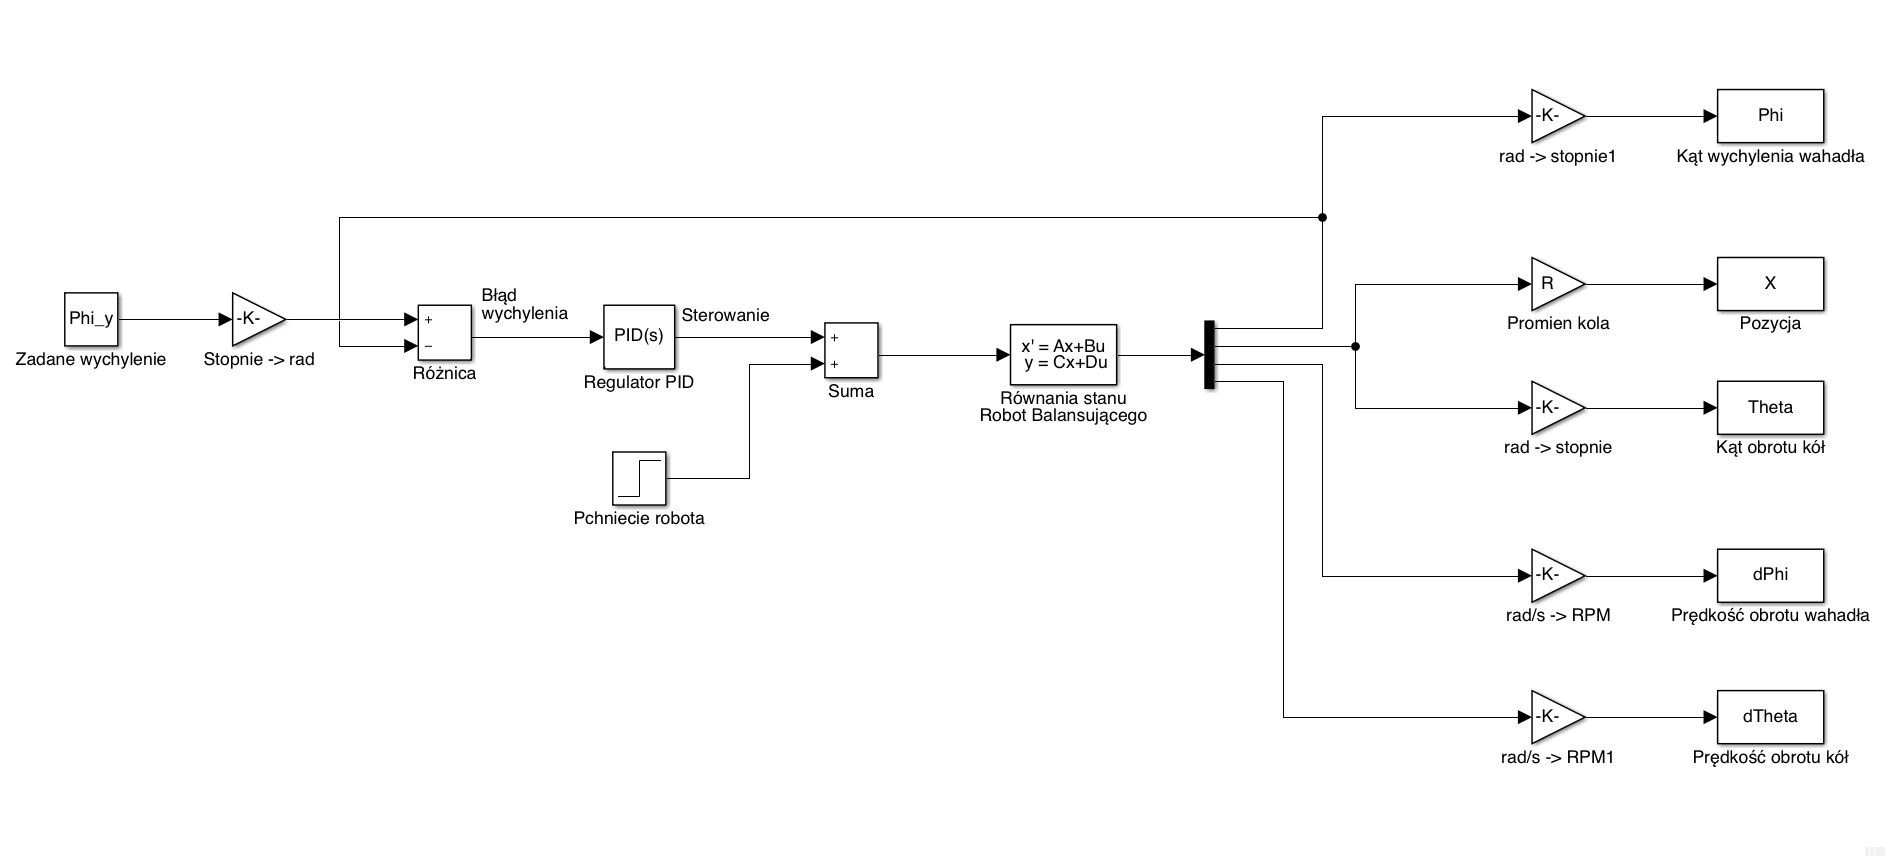
\includegraphics[width=0.9\textwidth]{Rysunki/Rozdzial02/Pojedynczy_PID.png}
	\caption{Schemat sterowania z wykorzystaniem jednego regulatora PID}
\end{figure}

W symulacji bloczki \texttt{gain} służą do przeliczenia radianów na stopnie oraz radiany na sekundę na liczbę obrotów na minutę. Są to jednostki bardziej przystępne i łatwiej sobie wyobrazić z jaką wartością mamy do czynienia.

Parametry regulatora wyznaczone zostały eksperymentalnie i prezentują się następująco
\begin{table}[h!]
    \centering
    \begin{tabular}{|c|c|}
        \hline
        $K_p$ & 10 \\
        \hline
        $K_i$ & 100 \\
        \hline
        $K_d$ & 0.1 \\
        \hline
        Wejście & Zadana prędkość kół \\
        \hline
        Wyjście & Zadany kąt wychylenia \\
        \hline
    \end{tabular}
        
    \caption{Parametry regulatora PID}
    \label{Parametry PID}
\end{table}

\begin{figure}
    Wizualizację tego jak zachowuje się wahadło podczas implementacji algorytmu i strojenia regulatora, daje prosta animacja pozycji kół oraz wychylenia wahadła. Na obrazku widzimy, że pomimo utrzymanego wychylenia wahadła w zadanej pozycji, położenie obiektu dryfuje w nieskończoność przy nieskończonym czasie symulacji.
    \\ 
    \begin{center}
        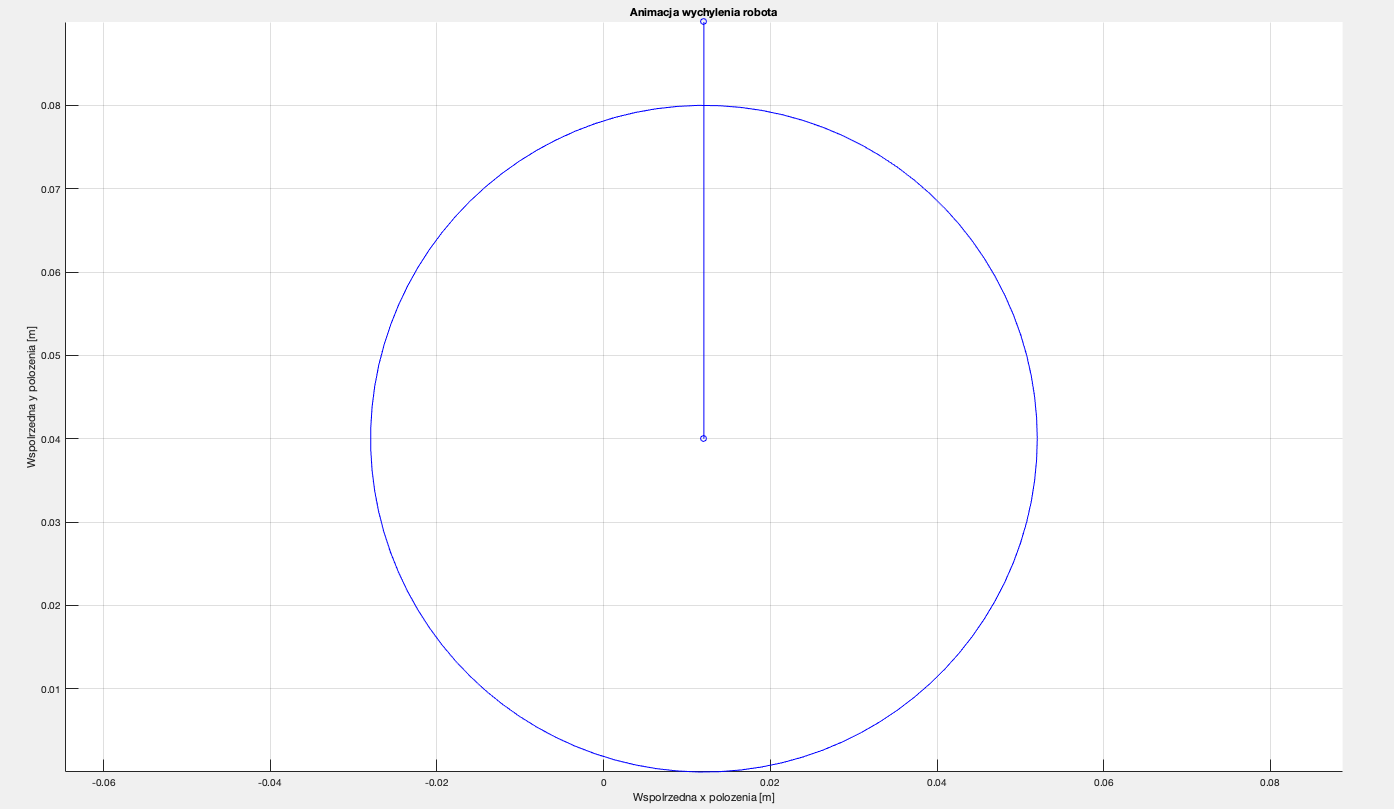
\includegraphics[width=0.9\textwidth]{Rysunki/Rozdzial02/Pojedynczy_PID_animacja.png}
	    \caption{Pozycja wahadła po 2 sekundach symulacji w płaszczyźnie XY}
    \end{center}
	\label{PID animacja}
\end{figure}

\begin{figure}
    Na początku symulacji wahadło znajduje się w punkcie równowagi, po czym w 1 sekundzie następuje skok jednostkowy, który symuluje pchnięcie robota generujące moment obrotowy o wartości 1 Nm. Takie wymuszenie wychyla wahadło w szczytowym momencie do wartości około 1.6 stopnia, oraz zmusza napęd do wygenerowania prędkości obrotowej kół na poziomie około 20 RPM. Jak widać na wykresie, czas stabilizacji wynosi około 0.4 s, przy czym pozycja robota zbiega do nieskończoności.
    \\
    \begin{center}
        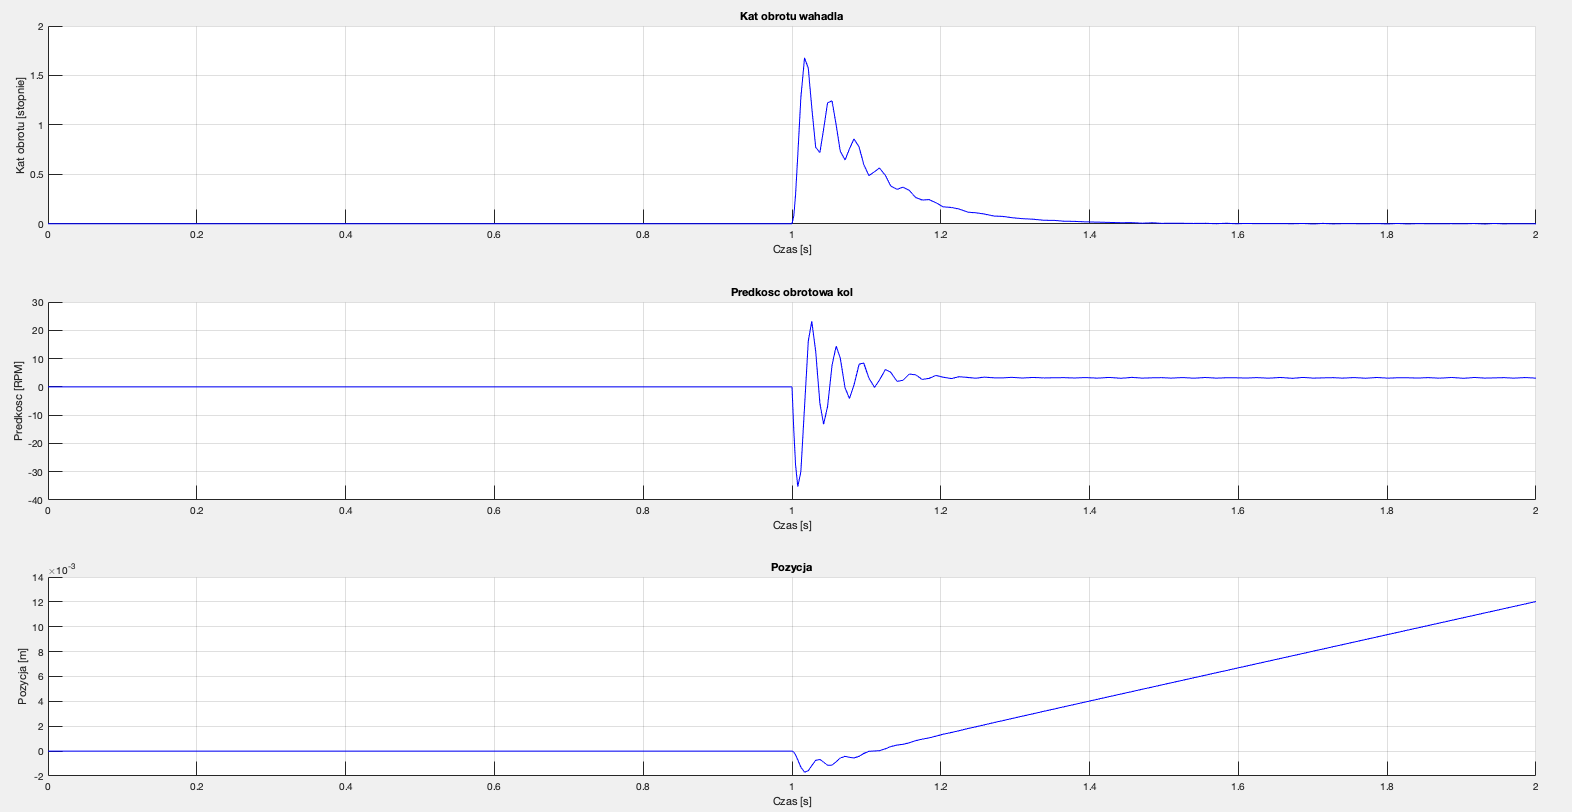
\includegraphics[width=0.9\textwidth]{Rysunki/Rozdzial02/Pojedynczy_PID_wykresy.png}
	    \caption{Wykres dla układu z jednym regulatorem: nr.1 -- wychylenie wahadła, nr.2 -- prędkość obrotu kół, nr.3 -- pozycja kół}
    \end{center}
	\label{Wykresy PID1}
\end{figure}

\newpage

\subsection{Podwójny regulator PID}
W przypadku, w którym zadaniem algorytmu jest nie tylko utrzymanie wychylenia wahadła, ale również utrzymanie zadanej pozycji czy prędkości kół, to pojawia się problem, ponieważ układ jest niedosterowany (dwie wielkości regulowane i jedno wymuszenie), który rozwiązuje zastosowanie dwóch regulatorów PID połączonych kaskadowo. Pierwszy regulator odpowiedzialny jest za utrzymanie zadanej prędkości kół lub pozycji, a drugi za utrzymanie prawidłowego kąta wychylenia wahadła. 

\begin{figure}[h!]
    \centering
	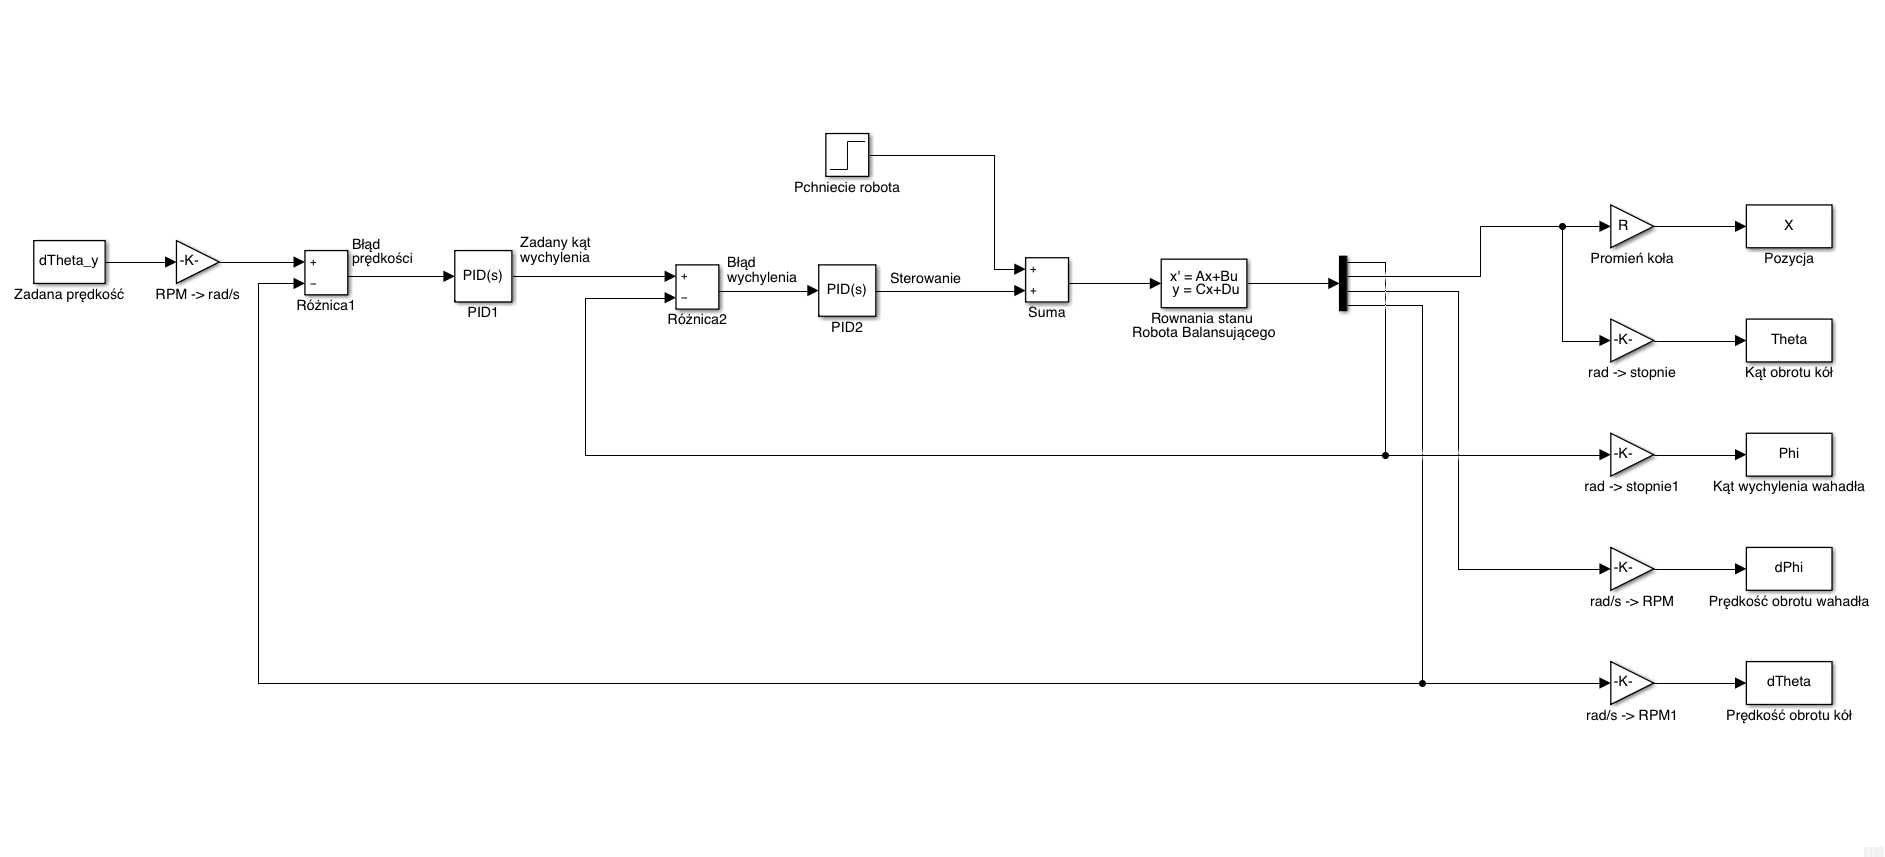
\includegraphics[width=0.9\textwidth]{Rysunki/Rozdzial02/Podwojny_PID.png}
	\caption{Schemat sterowania z wykorzystaniem dwóch regulatorów PID połączonych kaskadowo}
\end{figure}

Dla kaskadowego połączenia regulatorów, nastawy również zostały dobrane eksperymentalnie. Nastawy regulatora odpowiedzialnego za utrzymanie kąta wychylenia wahadła pozostały identyczne, jak w przypadku układu z pojedynczym regulatorem.
\begin{table}[h!]
    \centering
    \begin{tabular}{|c|c|}
        \hline
        $K_p$ & 20 \\
        \hline
        $K_i$ & 25 \\
        \hline
        $K_d$ & 0.02 \\
        \hline
        Wejście & Zadana prędkość kół \\
        \hline
        Wyjście & Zadany kąt wychylenia \\
        \hline
    \end{tabular}
        
    \caption{Parametry regulatora PID1}
    \label{Parametry PID1}
\end{table}

\begin{table}[h!]
    \centering
    \begin{tabular}{|c|c|}
        \hline
        $K_p$ & 10 \\
        \hline
        $K_i$ & 100 \\
        \hline
        $K_d$ & 0.1 \\
        \hline
        Wejście & Zadany kąt wychylenia \\
        \hline
        Wyjście & Sterowanie \\
        \hline
    \end{tabular}
        
    \caption{Parametry regulatora PID2}
    \label{Parametry PID2}
\end{table}

\begin{figure}[h!]
    Zadana prędkość kątowa kół równa zeru, sprawia że wahadło utrzymuje się w punkcie równowagi oraz wyeliminowano efekt dryfowania pozycji.
    \\ \\
    \begin{center}
        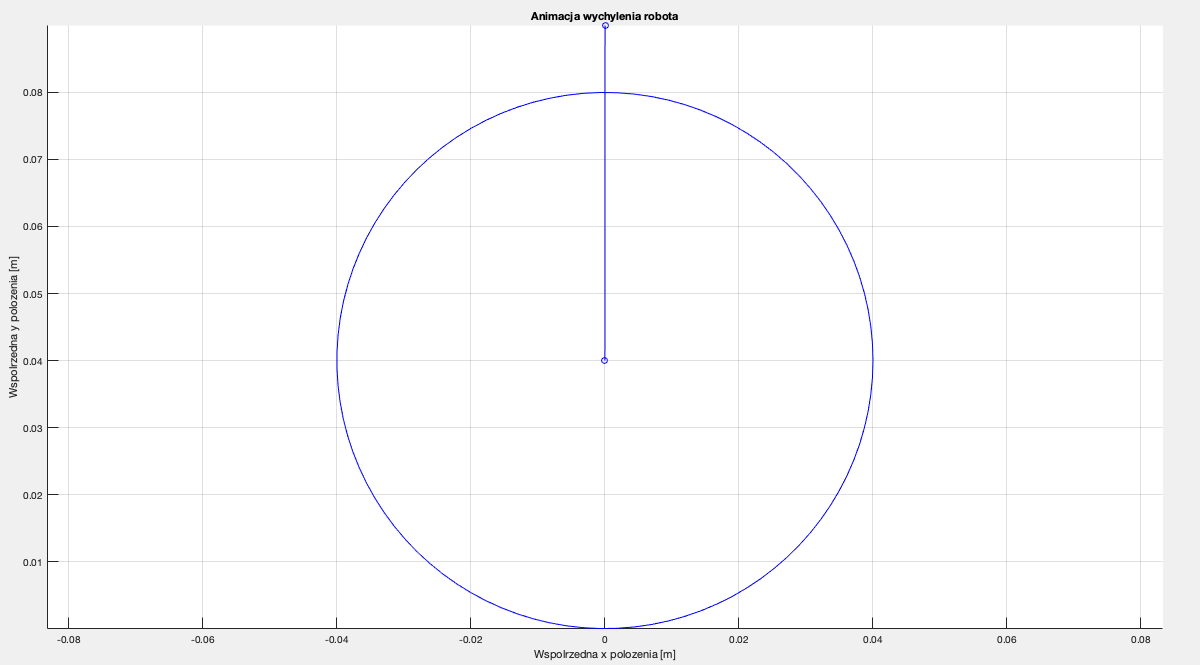
\includegraphics[width=0.9\textwidth]{Rysunki/Rozdzial02/Podwojny_PID_animacja.png}
	    \caption{Pozycja wahadła po 5 sekundach symulacji w płaszczyźnie XY}
    \end{center}
\end{figure}

\begin{figure}[h!]
    Jednym z efektów ubocznych zastosowania bardziej skomplikowanego układu regulacji jest wydłużenie samego czasu stabilizacji kąta wychylenia wahadła, co jest widoczne na wykresie.
    \\ \\ 
    \begin{center}
        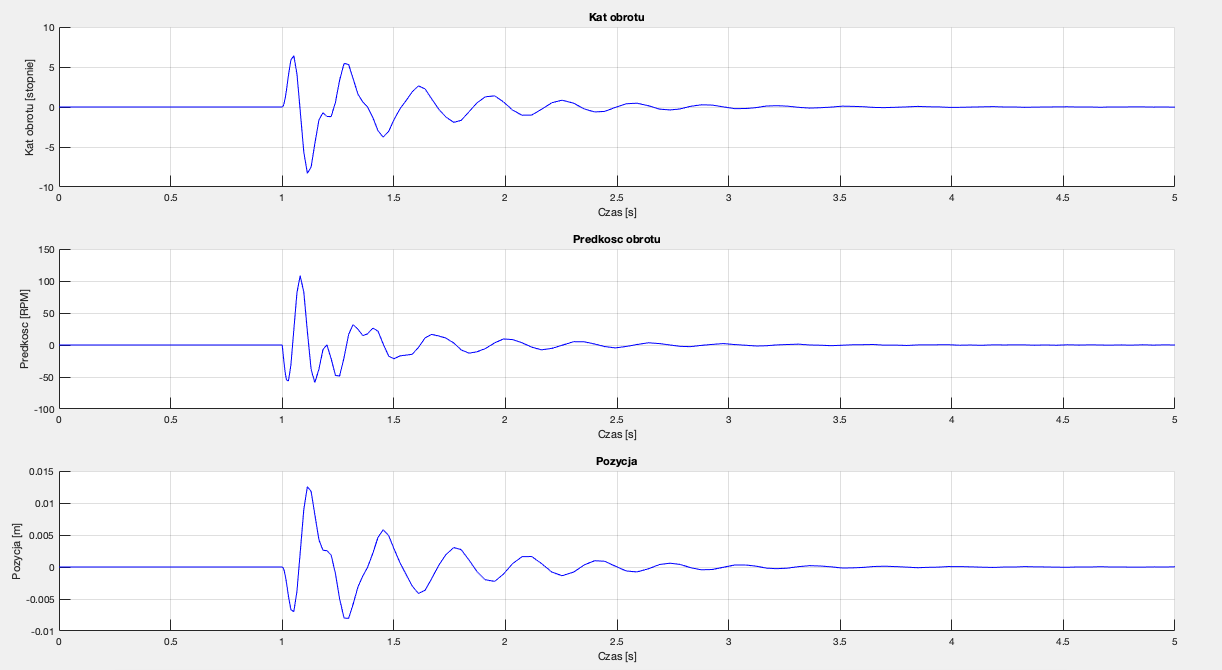
\includegraphics[width=0.9\textwidth]{Rysunki/Rozdzial02/Podwojny_PID_wykresy.png}
	    \caption{Wykres dla układu z dwoma regulatorami: nr.1 -- wychylenie wahadła, nr.2 -- prędkość obrotu kół, nr.3 -- pozycja kół}
    \end{center}
	\label{Wykresy PID2}
\end{figure}